\section{Les différentes stratégies de jeu}


\subsection{La stratégie aléatoire}
La stratégie aléatoire consiste à proposer un coup objectivement parmi les coups possibles. S'il arrive qu'il débute la partie, le coup qu'il propose est également aléatoire sinon, il accepte toujours le coup joué par l'adversaire.
Ainsi, le principe algorithmique sur lequel repose la stratégie aléatoire est le suivant: 
\\

\begin{algorithm}[H]
 \KwData{Le dernier coup \textbf{pm} du joueur adverse}
 \KwResult{Le coup \textbf{nm} du joeur aléatoire}

marquer dans le graphe le coup du joueur adverse;\\    
choisir aléatoirement un noeud \textbf{nm} quelconque du plateau jeu\\
\While{le noeud \textbf{nm} est occupé}{
    choisir aléatoirement un autre noeud \textbf{nm} \\
    }
colorer dans le graphe le noeud choisi;\\
retourner le noeud

\caption{Principe algorithmique du coup aléatoire}
\label{algoAléatoire}
\end{algorithm}

\subsection{La stratégie du bloqueur}

Le joueur qui utilise cette stratégie de jeu a pour but de bloquer les coups de son adversaire. En effet, comme l'adversaire essaye de joindre les deux bords du plateau correspondant à sa couleur par un chemin continue, l'objectif du bloqueur est de mettre un obstacle devant chacun de ses coups joués.
Cependant le choix des noeuds à occuper dépend de la couleur avec la quelle joue le client stratège.
Considérons par exemple un graphe hexagonale comme schématisé sur la figure 3:
\begin{itemize}
    \item Si le bleu représente l'adversaire, bloquer son coup revient à choisir l'un des noeuds blancs(C'est celui de gauche qui est généralement choisit). S'il arrive qu'ils soient occupés, le joueur rouge choisit un parmi les noeuds marrons mais généralement c'est le premier à gauche qui est choisit.
    
    \item Par contre si le rouge représente l'adversaire, la stratégie est de privilégier les noeuds marrons aux noeuds blancs.
\end{itemize}
S'il s'avère que tous les voisins du coup joué par l'adversaire sont colorés, le joueur propose aléatoirement un coup parmi ceux possibles.
\begin{figure}[h]
    \centering
    \label{fig:coupbloqueur}
    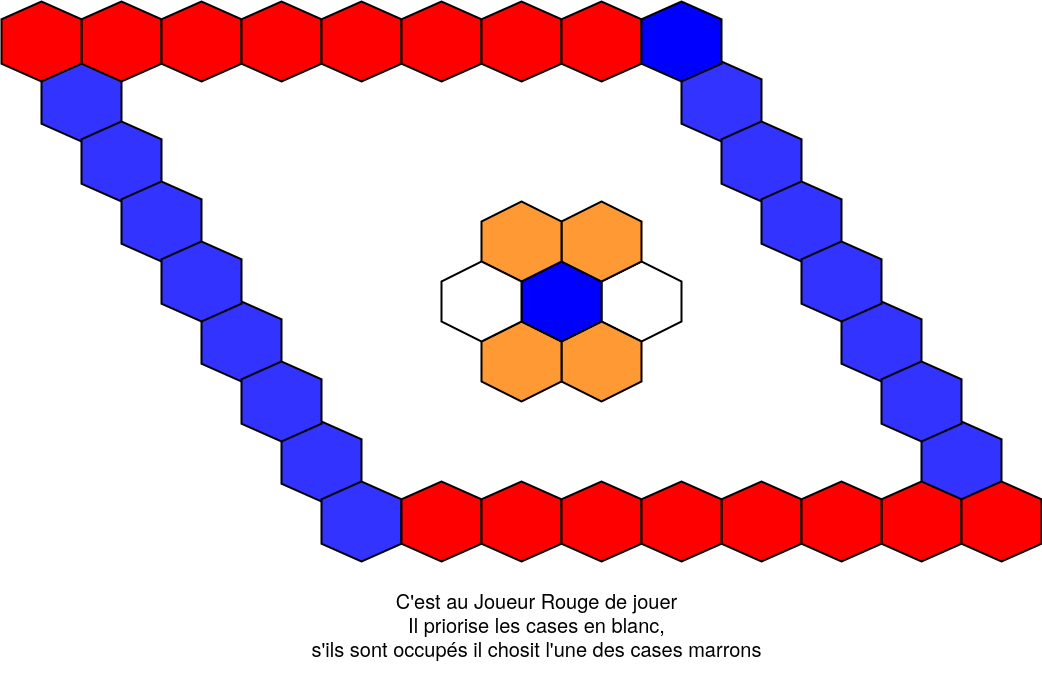
\includegraphics[width=0.4\textwidth]{Images/rouge.png}
    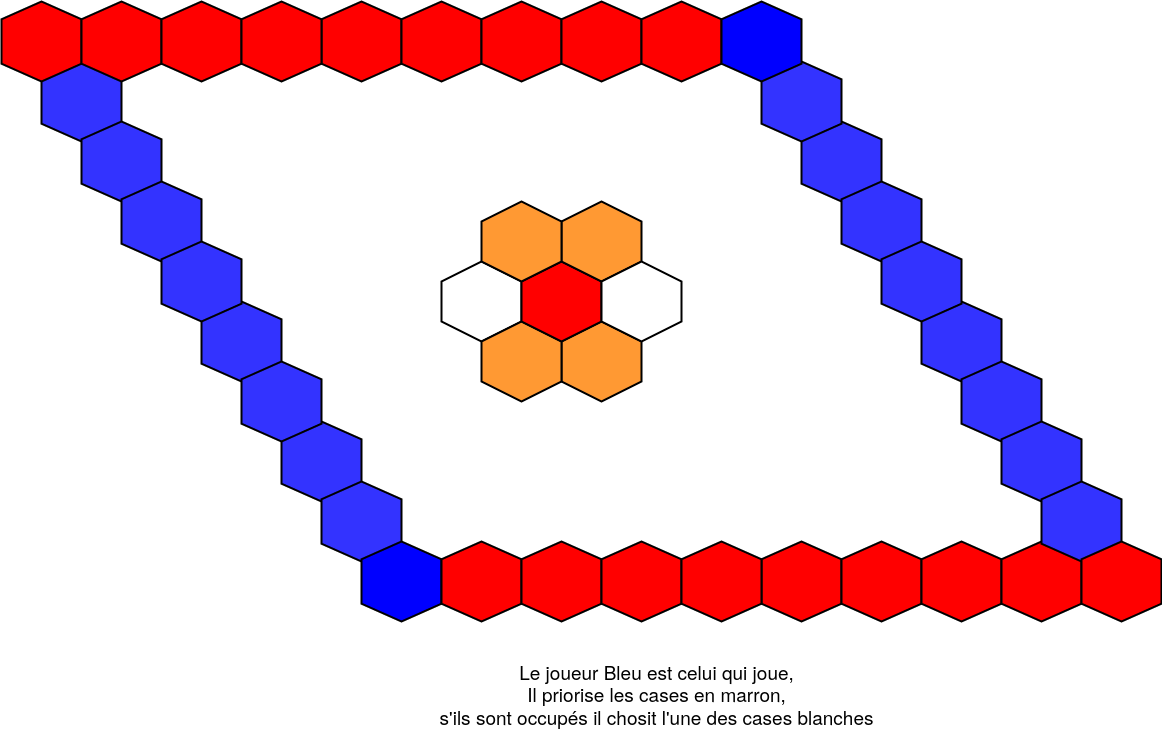
\includegraphics[width=0.4\textwidth]{Images/bleue.png}
    \caption{Choix du noeud obstacle}
\end{figure}

Ainsi, le principe algorithmique sur lequel repose cette stratégie est le suivant:
\begin{algorithm}[H]
 \KwData{Le dernier coup \textbf{pm} du joueur adverse}
 \KwResult{Le coup \textbf{nm} du joeur aléatoire}

marquer dans le graphe le coup \textbf{pm} joué par l'adversaire;\\   
Soit T un ensemble vide;\\
T $\leftarrow$ tous les noeuds inoccupés qui sont voisins à \textbf{pm};\\
\eIf{T n'est pas vide}{
    \eIf{Le joueur qui joue est le rouge}{
    privilégier le noeud de gauche et celui de droite du noeud rouge;\\
    s'ils sont colorés choisir un noeud non coloré parmi les quatre autres;\\}{
    privilégier les noeuds placés au dessus et en dessous du noeud bleu;\\
    s'ils sont tous occupés, choisir soit celui de gauche ou celui de droite;\\}}
    {
    choisir aléatoirement un noeud inoccupée}
colorer dans le graphe le noeud choisi;\\
retourner le noeud

\caption{Principe algorithmique de la stratégie du bloqueur}
\label{algoBi}
\end{algorithm}

\subsection{la stratégie du coup maintenant le plus court chemin}
Cette stratégie se base essentiellement sur le maintien du plus court chemin après chaque coup joué par l'adversaire. En effet une structure stratégie est nécessaire pour stocker les indices des bords du plateau au début du jeu qui permettront de déterminer à chaque fois le chemin le plus court à travers le fameux algorithme \textit{DIJSKTRA}. A chaque fois qu'un chemin est généré on suppose que $n$ est la distance ou bien le nombre de cases restantes pour ce chemin, à ce stade pour trouver le prochain coup, on colore chaque case du chemin par la couleur de l'adversaire si jamais on ne trouve pas un chemin alternative de profondeur n, donc cette case colorée est la seule à avoir maintenu la notion du plus court chemin, c'est bien la case à jouer.

\begin{figure}[h]
    \centering
    \label{fig:Hexmove}
    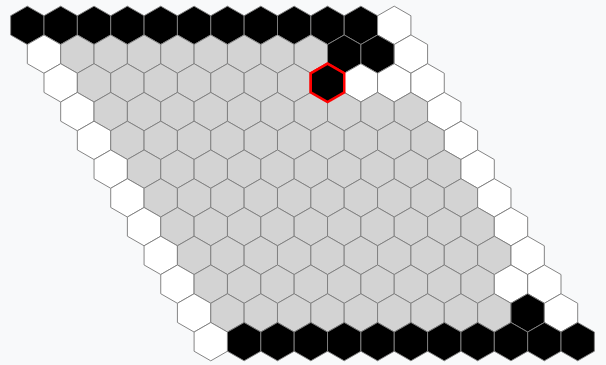
\includegraphics[width=0.85\textwidth]{Images/Hex_move_shortest.png}

    \caption{Prochain coup généré par l'algorithme pour le joueur noir}
\end{figure}

La figure \ref{fig:Hexmove} montre le coup choisi par l'algorithme, avant de jouer le coup choisi entouré en rouge, le plus court chemin était de profondeur 9, et ce coup étant un parmi les coups minimisants la profondeur du plus court chemin, mais étant le seul à avoir garder plus de 2 chemins de profondeur 8 par suite, en supposant n'importe quel prochain coup de l'adversaire dans le cas de la figure \ref{fig:Hexmove} le joueur garde toujours un second chemin de profondeur 8 à suivre.\\

\begin{algorithm}[H]
 \KwData{Tablier du jeu \textbf{T}, Couleur du joueur \textbf{c}}
 \KwResult{Le coup \textbf{n}}

$Chemin \leftarrow$ plus court chemin entre les deux bords colorés en \textbf{c} de \textbf{T};\\
$profondeur \leftarrow$ $taille(chemin)$; \\    
\If{$Chemin\ est\ vide$}{
    $n \leftarrow$ coup aléatoire valide ;
}
\While{$Chemin\ ! vide$}{
    $n \leftarrow$ noeud du Chemin;\\
    Retirer $n$ du Chemin;\\
    Colorer le noeud $n$ par la couleur inverse de \textbf{c};\\
    $alternative \leftarrow$ plus court chemin entre les deux bords;\\
    \If{$profondeur < taille(alternative)$}{
        \textbf{break}
        \\}}
colorer dans le graphe $n$ choisi par la couleur \textbf{c};\\
retourner n;

\caption{Principe algorithmique du coup maintenant le plus court chemin}
\label{algoShortPath}
\end{algorithm}
La complexité de l'algorithme est \textbf{quadratique} en nombre de sommets, dû à celle de \textit{Dijsktra} implémenté en utilisant des tableaux. Ce qui demande un temps raisonnable au joueur pour répondre au coup de l'adversaire.

\subsection{la stratégie "two-distances"}
La stratégie implémenté basée sur le principe du deux-distances \textit{(two-distances, van Rijswijck, 2000)} est fournit principalement par l'algorithme \textit{Minimax}. En effet,\textit{two-distances} est une façon d'évaluer un tablier. En l'évaluant, on peut déterminer le joueur qui est susceptible de gagner. Le problème avec la stratégie précédente c'est que si l'adversaire bloque le joueur un peu plus loin, le joueur n'a aucune information sur l'existence de son plus court chemin et du chemin alternatif, d'où l'idée d'évaluer plus de positions.
\subsubsection{Méthode de Minimax}
La stratégie minimax détermine les valeurs des positions du tablier non terminales ou détermine de nouvelles positions terminaux. L'algorithme suppose un jeu optimal alternatif des deux côtés et recherche les branches de l'arbre vers les nœuds terminaux, ou  jusqu'à une profondeur donnée. Dans le cas du jeu de Hex la taille du tablier ne permet pas d'aller jusqu'au bords, d'où la nécessité d'une fonction qui évalue un tablier avec quelques coups. 
\subsubsection{Évaluation "two-distances"}
La fonction d'évaluation \textit{two-distances} est basée sur la mesure de la connectivité relative d'une position Hex, et qui prend en considération la présence des chemin alternatifs. Son principe définit la distance $d(u,v)$ pour deux sommets $u$ et $v$ comme suit:
\begin{equation}
    d(u,v) = 1\ ,\ Si\ u\ et\ v\ sont\ voisins. \\
\end{equation}
Sinon, en supposant $N(u)$ l'ensemble des voisins de $u$, et en retirant $u'$ le voisin de $u$ de plus proche distance de v, on considère un nouveau voisin $u'' \in N(u)$ le plus proche de v, et on définit:
\begin{equation}
    d(u,v) = 1 + d(u'',v)
\end{equation}
Alors, en considérant $e_{1p}$ $e_{2p}$ deux sommets appartenant respectivement aux deux bords du tablier de la même couleur pour un joueur $p$, la fonction d'évaluation du tableau $f$ est la distance entre les deux sommets: \\
\begin{equation}
    f(p) = d(e_{1p},e_{2p})
\end{equation}

\subsubsection{Principe implémenté}
Le principe implémenté et décrit par l'algorithme \ref{algominimax} consiste à minimiser la distance entre les deux bords du tablier du joueur en jouant un coup. Par l'algorithme de \textit{minimax}, on souhaite évaluer les noeuds du tablier, l'évaluation d'un noeud dans un tablier vide de forme hexagonale coûte $\mathcal{O} (6^{d}\times c) $, où $c$ est la complexité de la fonction d'évaluation, $d$ la profondeur souhaitée lors de l'utilisation de \textit{mimimax}. En effet, une grande complexité résulte de la fonction d'évaluation où on utilise \textit{DIJSKTRA} pour trouver les voisins $u'$ et $u"$ ce qui rend l'algorithme plus complexe.\\
Alors, afin de minimiser le temps de calcul du joueur, un choix optimal des noeuds évalués est fait, il consiste à ne prendre en considération que l'ensemble des noeuds définissant l'intersection des plus courts chemins pour chaque joueur.\\ \\
\begin{algorithm}[H]
 \KwData{Tablier du jeu \textbf{T}, Couleur du joueur \textbf{c}, Profondeur \textbf{p}, Fonction d'évaluation \textbf{f}}
 \KwResult{Le coup \textbf{n}}

$Chemin1 \leftarrow$ plus court chemin entre les deux bords colorés en \textbf{c} de \textbf{T};\\
$Chemin2 \leftarrow$ plus court chemin entre les deux bords colorés en \textbf{{c}} de \textbf{T};\\
$Region \leftarrow Chemin1 \cap Chemin2 $; \\    
\eIf{$Region\ est\ vide$}{
    $n \leftarrow$ coup aléatoire valide ;
}{
$n \leftarrow Minimax(T,p,-\infty,+\infty,Region,Minimisation,f)$
}
colorer dans le graphe $n$ choisi par la couleur \textbf{c};\\
retourner \textbf{n};

\caption{Principe algorithmique du coup évalué par Minimax à travers l'évaluation $f$}
\label{algominimax}
\end{algorithm}


La fonction \textit{Minimax} utilisée est optimisée par l'élagage alpha-Beta, ce sont les deux paramètres initialisés lors de l'appel de \textit{Minimax} en $+\infty$ et $-\infty$, le paramètre $Minimisation$ est un booléen indiquant le souhait de la minimisation de la distance entre les deux bords pour ce joueur, $p$ c'est la profondeur du calcul.
